\documentclass[../report]{subfiles}
\setcounter{section}{0}
\begin{document}

本章では,本プロジェクトの活動プロセスを説明する.
\bunseki{堀沙枝香}

\section{活動スケジュール}
プロジェクト全体の活動及び医療グループの活動スケジュールを以下に記す.
\begin{itemize}
    \item[] 5月
    \begin{itemize}
        \item プロジェクト発足
        \item プロジェクトリーダー決定
        \item グループ分け
        \item グループリーダー決定
        \item キックオフイベント
        \item 南部先生によるフィールドワーク講座
        \item 認知症サポーター養成講座
        \item アイデアレビュー会
    \end{itemize}
    \item[] 6月
    \begin{itemize}
        \item 月例レビュー会
        \item 月例レビュー会の振り返り
        \item 石別フィールドワーク
        \item Skype会議
        \item ロボット開発ワークショップへの参加
        \item もの忘れカフェへの参加
        \item 中間成果発表ポスター作成開始
    \end{itemize}
    \item[] 7月
    \begin{itemize}
        \item 中間成果発表ポスターレビュー会
        \item 中間報告書作成開始
        \item 中間成果発表会
        \item 中間報告書提出
        \item 今後の活動についての話し合い
    \end{itemize}
\end{itemize}
\bunseki{堀沙枝香}

\section{活動概要}
\subsection{学習とシステム案の検討}\label{sec:kentou}
認知症の症状やその療法,認知症に関する現状の社会問題や取り組みを本やインターネットを利用して個人で調べた.
そこで得た知識をもとに,個人でシステム案を検討し,それぞれの案をグループ内で共有した.
案の内容については\ref{sec:andashi}で述べる.
また,システム案の検討と同時に,既存の認知症に関するデバイスやアプリについても調べた.
\bunseki{堀沙枝香}

\subsection{認知症サポーター養成講座}
函館認知症の人を支える会の方々を大学にお招きし,認知症とは何か,認知症を引き起こす原因,中核症状と行動・心理症状,認知症の人の支援の仕方などといった内容の講座を開いて頂いた.
その後,本グループで考えているシステムを提案し,それについてディスカッション形式でご意見を頂いた.
頂いたご意見を参考にして,システム案の修正を行った.頂いたご意見のについて詳しくは\ref{sec:review-sasaerukai}にて述べる.
\begin{figure}[htbp]
    \begin{center}
        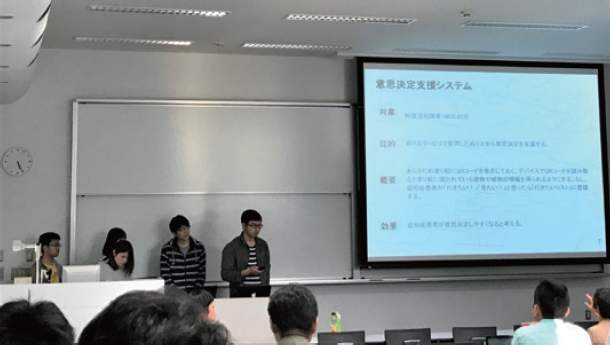
\includegraphics[width=10cm]{imgs/ninchisyo-kouza.png}
        \caption{認知症サポーター養成講座}
        \label{fig:ninchisyo-kouza}
    \end{center}
\end{figure}
\bunseki{堀沙枝香}

\subsection{認知症の臨床研究を行っている医師への提案}
認知症を専門に研究されている京都府立医科大学の成本医師と,Skypeを介して本グループで考えているシステムを提案し,一つ一つにご意見を頂いた.
頂いたご意見について詳しくは\ref{sec:review-narumoto}にて述べる.
その後,提案したシステム案の中で成本医師自身が気になったものを選んで頂き,その理由を伺った.
また,成本先生から事前に頂いていたキーワードの一つである「医療選択・意思決定支援」に必要としているものは何かを抽象的に尋ねた.
結果,医療従事者に提供される情報として望ましいものなど,今後システムを考える上で手がかりになるようなご意見を頂いた.
\begin{figure}[htbp]
    \begin{center}
        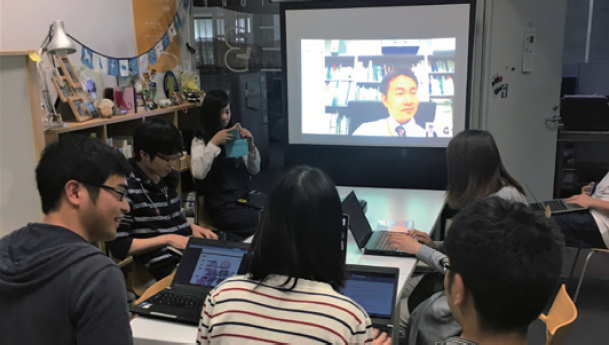
\includegraphics[width=10cm]{imgs/ninchisyo-kaigi.png}
        \caption{京都府立医科大学の成本医師とのSkype会議}
        \label{fig:ninchisyo-kaigi}
    \end{center}
\end{figure}
\bunseki{堀沙枝香}

\subsection{ロボット開発ワークショップ}
京都の同志社女子大学京田辺キャンパスで開催された,ロボット開発ワークショップに参加した.
このワークショップでは,自身の価値にまつわる過去の経験を説明し,他者とのコミュニケーションの中で互いの価値を見つけ出すという体験をした.
またこの体験から,ロボットが人間とのコミュニケーションの中で,価値を引き出す際に必要なものは何かを自身がロボットの立場になり考えた.
\begin{figure}[htbp]
    \begin{center}
        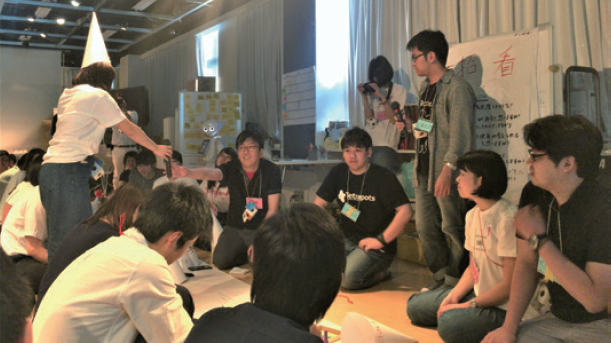
\includegraphics[width=10cm]{imgs/ninchisyo-ws.png}
        \caption{ロボット開発ワークショップ}
        \label{fig:ninchisyo-ws}
    \end{center}
\end{figure}
\bunseki{堀沙枝香}

\subsection{もの忘れカフェ}
函館認知症の人を支える会の方々が主催している,もの忘れカフェに参加した.
もの忘れカフェとは,物忘れで困っている人やそんな人たちを支えたい人たちが集まり,話をする場である.
そこでの対談する時間を利用して,ボランティアの方々に自己紹介も兼ねて,本グループの活動について紹介させて頂いた.
活動に興味を持ってくださったので,現状で考えているシステムについての説明をし,それについてご意見を頂いた.
頂いたご意見について詳しくは\ref{sec:review-monowasurecafe}で述べる.
\bunseki{堀沙枝香}

\subsection{システム案の再検討と方向性の決定}\label{sec:saikentou}
\ref{sec:kentou}で生まれたシステム案修正に試行錯誤が続いたため,建設的なアイデアが生まれることを期待し,\ref{sec:kentou}で考えたシステム案とは全く違う目線で今までに得た学びを踏まえ,案の再検討を試みた.
結果,「認知症になる前段階の高齢者に認知症の予防をさせること」,「ライフログデータを利用して見直しのきっかけづくりや意思決定支援に繋げること」といった方向性に決定し,「認知症予防のための食習慣改善システム」を提案した.
\bunseki{堀沙枝香}

\subsection{中間発表会}
\ref{sec:saikentou}で提案したシステムや活動プロセスを,中間発表会でポスターセッション形式にて発表した.
発表の際に頂いたご意見をまとめた結果,「高齢者への撮影した写真データの見せ方」,「料理の撮影方法」などのシステム内容に改善の余地があると考えた.
本グループはこれらの方法に対し,検討を試みる及び改善することを今後の課題として追加する.
\bunseki{堀沙枝香}

\end{document}
